\documentclass[12pt, a4paper]{article}
\usepackage[a4paper, top=2cm, bottom=3cm, left=2cm, right=2cm]{geometry}
\usepackage[export]{adjustbox}
\usepackage{graphicx}
\usepackage{mathtools}
\usepackage{hyperref}
\usepackage{amsmath}
\usepackage{amsfonts}
\usepackage{amssymb}
\usepackage[version=4]{mhchem}
\usepackage{stmaryrd}
\usepackage{polyglossia}
\usepackage{fontspec}
\usepackage{ucharclasses}
\usepackage{fancyhdr}
\usepackage{wrapfig}
\usepackage{subcaption}
\usepackage{relsize}
\usepackage{framed}
\usepackage{changepage}
\usepackage{tabularray}
\usepackage{etoolbox}
\usepackage{xstring}
\usepackage{pstricks-add}
\usepackage{tikz}
\usepackage{empheq}
\usepackage{tcolorbox}
\usepackage[european,s traightvoltages, americanresistor, americaninductors]{circuitikz}
\usepackage{pgfplots}
\usepackage{tikz-3dplot}

\usetikzlibrary{
	angles,
	arrows.meta,
	positioning,
	arrows,
	backgrounds,
	calc,
	decorations,
	decorations.markings,
	decorations.pathmorphing,
	fit,
	shapes.arrows,
	shapes.callouts,
	shapes.geometric,
	shapes.misc,
	snakes,
	quotes
}
\pgfplotsset{compat=1.18}
\hypersetup{colorlinks=true, linkcolor=blue, filecolor=magenta, urlcolor=cyan,}
\urlstyle{same}

\setmainlanguage{english}
\setotherlanguages{norwegian, arabic}
\newfontfamily\arabicfont{Noto Naskh Arabic}
% \newfontfamily\lgcfont{CMU Serif}

%%%%%%%%%% Fancy header %%%%%%%%%
\pagestyle{fancy}
\fancyhead[C]{}
\fancyfoot[C]{\medskip\thepage}
\renewcommand{\footrulewidth}{.4pt}
\renewcommand{\headrulewidth}{0pt}

\setlength{\headheight}{14.49998pt}
\addtolength{\topmargin}{-2.49998pt}

\newcommand{\figwidth}{8cm}
\newcommand{\floatfigwidth}{5cm}


%%%%%%%%%% Formatters & Layout %%%%%%%%%
\newcommand{\uprimary}[1]{
	\section*{\center \Huge \underline{#1}}
	\addcontentsline{toc}{section}{\protect\numberline{}#1}
}
\newcommand{\usecondary}[1]{
	\section*{\center \LARGE \underline{#1}}
	\addcontentsline{toc}{section}{\protect\numberline{}#1}
}
\newcommand{\usection}[1]{
	\section*{\LARGE #1}
	\addcontentsline{toc}{subsection}{\protect\numberline{}#1}
}
\newcommand{\usubsection}[1]{
	\section*{\Large #1}
	\addcontentsline{toc}{subsection}{\protect\numberline{}#1}
}
\newcommand{\ussubsection}[1]{
	\section*{\large #1}
	\addcontentsline{toc}{subsection}{\protect\numberline{}#1}
}
\newcommand{\ans}{\bigskip\underline{\textbf{Answer}}}
\newcommand{\ques}[1]{\noparindent\textbf{#1}\doparindent}
\newcommand{\rfloatingimg}[1]{
	\begin{wrapfigure}{r}{\floatfigwidth}
		\includegraphics[max width=\floatfigwidth]{#1}
	\end{wrapfigure}
}
\newcommand{\indentbox}[2]{
	\begin{adjustwidth}{#1}{0pt}
		#2
	\end{adjustwidth}
}
\newcommand{\qa}[3]{
	\noparindent
	\textbf{#1 #2}
	\indentbox{.76cm}{
		\ans
		#3
	}
	\vspace{.75cm}
}
\newcommand{\noskipqa}[2]{
	\noparindent
	\textbf{#1}
	\indentbox{.76cm}{
		\ans
		#2
	}
}
\newcommand{\eqnleft}[1]{
	\begin{flalign*}
		 & #1 &  &
	\end{flalign*}
}
\newcommand{\fullwidthimg}[1]{
	\begin{center}
		\includegraphics[max width=\textwidth]{#1}
	\end{center}
}
\newcommand{\uheading}[2]{
	\uprimary{Module - #1}
	\vspace{-.7cm}
	\usecondary{#2}
}

\newcommand{\note}[1]{
	\begin{tcolorbox}[colframe=green!40!black, colback=green!5!white, title={\textbf{Note}}]
	#1
	\end{tcolorbox}
}


%%%%%%%%%% general constants/symbols %%%%%%%%%
\newcommand\longUparrow{\mathrel{\scalebox{1}[2]{$\uparrow$}}}
\DeclareRobustCommand{\rchi}{{\mathpalette\irchi\relax}}
\newcommand{\irchi}[2]{\raisebox{\depth}{$#1\chi$}}
\newcommand{\term}[1]{\underline{\textbf{#1}}}
\newcommand{\amstr}{\mathring{\textrm{A}}}
\newcommand{\h}{6.626 \times 10^{-34}}
\newcommand{\kB}{1.38 \times 10^{-23}}
\newcommand{\lc}{3 \times 10^{8}}
\newcommand{\uunit}[1]{\mathrm{~#1}}

%%%%%%%%%% Format constants %%%%%%%%%
\newcommand{\doparindent}{\setlength\parindent{.5cm}}
\newcommand{\noparindent}{\setlength\parindent{0pt}}
\graphicspath{ {../images/} }
\NewDocumentCommand{\multiskip}{m}{%
	\begingroup
	\newcount\i  % Define a new counter \i
	\i=0         % Initialize the counter
	\loop
	\ifnum\i<#1
	\bigskip  % Add \bigskip
	\advance\i by 1  % Increment the counter
	\repeat
	\endgroup
}

\newcommand{\termlist}[1]{
	\begin{tcolorbox}[colback=blue!10!white, colframe=blue!50!black, title={Some terms}]
		#1
	\end{tcolorbox}
}


%%%%% dev fx
% startx, starty, endx, endy
\newcommand{\dottedgrid}[4]{
	\draw[thin, dotted] (#1, #2) grid (#3,#4);
	\foreach \i in {#1,...,#3} \node at (\i,-2ex) {\i};
	\foreach \i in {#2,...,#4} \node at (-2ex,\i) {\i};
}
\newcommand{\smallmidarrow}[2]{\tikz \draw[arrows = {-Straight Barb[scale=.8]}, line width=#1] (0,0) -- +(#2,0);}
\newcommand{\midarrow}[2]{\tikz \draw[arrows = {-Straight Barb[scale=1.1]}, line width=#1] (0,0) -- +(#2,0);}

\DefTblrTemplate{caption-tag}{default}{}
\DefTblrTemplate{caption-sep}{default}{}
\DefTblrTemplate{caption-text}{default}{}
\DefTblrTemplate{contfoot-text}{default}{}
\DefTblrTemplate{conthead-text}{default}{}
\usepackage{tikz}

\graphicspath{ {../images/} }

\begin{document}
\uheading{1}{Lasers \& Fibre optics}
\usection{Laser}
$\sim$ Light amplification by stimulated emission of radiation
- (others: Maser, Eraser).

\usubsection {Characteristics}

\begin{enumerate}
	\item \term{Monuchromaticity}\\
	      Has extremely narrow bandwidth. $\Delta \lambda=5 \times 10^{-14} \unit{m}$ (conventional light source: 1000 $\amstr$)\\
	      Degree of monochromaticly: $\varepsilon=\frac{\Delta\lambda}{\lambda}$ \ \ ($\Delta\lambda \Rightarrow$ spead of light)
	\item \term{Directionality}\\
	      Can travel large distances with minimal deviation.\\
	      Divergence $\Delta \theta=\frac{r_2-r_1}{D_2-D}$ or $D^2 / \lambda$ (Reliegh's range) \\
	      For laser: $10 \mu\unit{rad}$\\
	      for search light $0.5rad$
	      $>\Rightarrow$ divergence
	\item \term{Coherence}\\
	      \textbf{Spatial coherence}:when a when wave maintains constant phase difference at two points on the wave over a time ($t$).

	      \textbf{Temporal coherence}: when there is no phase change at a point on the wave over a time. (these reference points are taken on electric field)
	\item \term{Brightness/intensity}\\
	      Laser produce highly intense beams, because more light energy is concentrated in a small region. Also laser light is coherent, so at a time many photons are in phase. They superimpose to produce a wave of larger amplitude. Hence resultant intensity  $\propto$amplitude$^2$) is very high.
\end{enumerate}

\noparindent
\begin{framed}
	\indentbox{0.75cm}{
	\term{Coherence length ($L_c$)}:Propagation distance over which a coherent wave maintains a specified degree of coherence or phase difference \\
	for He-Ne: 600km


	\term{Coherence time($\tau_c$)}: time over which a propagating wave remains coherent or the maximum time interval for which the wave have definite phase relation. \\
	For He-Ne: $\tau_c=2 \times 10^{-3} \unit{s}$\\
	Sodium lamp: $10^{-10} \unit{s}$\\
	\term{non-chromaticity $\propto L_c^{-1}$}
	}
\end{framed}

\newpage
\usubsection{Spontaneous \& stimulated emission}

\bigskip

\begin{center}
	\begin{tikzpicture}[scale=.9]

		\coordinate (E1) at (0, 0);
		\coordinate [above=3 of E1] (E2);

		\coordinate [right=.4 of E1] (E1t);
		\coordinate [right=.4 of E2] (E2t);

		\draw[thick] (E1t) --++ (0:5) coordinate (Ee1);
		\draw[thick] (E2t) --++ (0:5) coordinate (Ee2);

		\path[black] (E1) node{$\textrm{E}_1$};
		\path[black] (E2) node{$\textrm{E}_2$};

		\fill[black] ($(E2t)!.5!(Ee2)$) circle(3pt);

		\draw[thick, ->] ($($(E1t)!.5!(E2t)$) + (0:6)$) --++(0:1);

		\begin{scope}[xshift=9cm,decoration={snake}]
			\coordinate (E1) at (0, 0);
			\coordinate [above=3 of E1] (E2);

			\coordinate [right=.4 of E1] (E1t);
			\coordinate [right=.4 of E2] (E2t);

			\draw[thick] (E1t) --++ (0:5) coordinate (Ee1);
			\draw[thick] (E2t) --++ (0:5) coordinate (Ee2);

			\path[black] (E1) node{$\textrm{E}_1$};
			\path[black] (E2) node{$\textrm{E}_2$};

			\fill[black] ($(E1t)!.5!(Ee1)$) circle(3pt);

			\draw[-{Latex[length=3mm]}] ($(E2t)!.5!(Ee2)$) coordinate (x1) -- ($($(E1t)!.5!(Ee1)$)+(0,.15)$) coordinate (x2);
			\draw[thick,decorate,red,->] ($($(x1)!.5!(x2)$) + (0:.2)$) coordinate (y1) -- node [above,align=left,yshift=1mm,font=\footnotesize] {$h\nu$} ($(y1) + (0:1)$);

			\node[align=center] at ($(y1)+(0:4)$) {Spontaneous \\ Emission};
		\end{scope}

	\end{tikzpicture}

	\multiskip{5}

	\begin{tikzpicture}[decoration={snake}, scale=.9]

		\coordinate (E1) at (0, 0);
		\coordinate [above=3 of E1] (E2);

		\coordinate [right=.4 of E1] (E1t);
		\coordinate [right=.4 of E2] (E2t);

		\draw[thick] (E1t) --++ (0:5) coordinate (Ee1);
		\draw[thick] (E2t) --++ (0:5) coordinate (Ee2);

		\path[black] (E1) node{$\textrm{E}_1$};
		\path[black] (E2) node{$\textrm{E}_2$};

		\fill[black] ($(E2t)!.5!(Ee2)$) circle(3pt);

		\draw[thick,decorate,red,->] ($($(E1t)!.5!(E2t)$) + (.4, 0)$) coordinate (y1) -- node [above,align=left,yshift=1mm,font=\footnotesize] {$h\nu$} ($(y1) + (1, 0)$);
		\draw[thick, ->] ($($(E1t)!.5!(E2t)$) + (0:6)$) --++(0:1);

		\begin{scope}[xshift=9cm,decoration={snake}]
			\coordinate (E1) at (0, 0);
			\coordinate [above=3 of E1] (E2);

			\coordinate [right=.4 of E1] (E1t);
			\coordinate [right=.4 of E2] (E2t);

			\draw[thick] (E1t) --++ (0:5) coordinate (Ee1);
			\draw[thick] (E2t) --++ (0:5) coordinate (Ee2);

			\path[black] (E1) node{$\textrm{E}_1$};
			\path[black] (E2) node{$\textrm{E}_2$};

			\fill[black] ($(E1t)!.5!(Ee1)$) circle(3pt);

			\draw[-{Latex[length=3mm]}] ($(E2t)!.5!(Ee2)$) coordinate (x1) -- ($($(E1t)!.5!(Ee1)$)+(0,.15)$) coordinate (x2);
			\draw[thick,decorate,red,->] ($($(x1)!.5!(x2)$) + (.2, 0)$) coordinate (y1) -- node [above,align=left,yshift=1mm,font=\footnotesize] {$2h\nu$} ($(y1) + (1,0)$);
			\draw[thick,decorate,red,->] ($(y1) + (0,-.2)$) coordinate (y1) -- ($(y1) + (0:1)$);

			\node[align=center] at ($(y1)+(0:4)$) {Stimulated \\ Emission};
		\end{scope}

	\end{tikzpicture}
\end{center}

\ussubsection{Spontaneous emission}
Atom initially at excited state makes transition voluntarily on its own, without aid of any external agency, to ground state, and emits photon of energy $$h \nu_{12}=E_2-E_1$$
Different atoms of medium emits light at different times and different directions. Hence emitted photons are incoherent. The rate of emission is independent of incident energy (as no energy is supplied to the system.)

\ussubsection{Stimulated emission}
Here photon having energy $h\nu_{12}(=E_2-E_1)$ impinges on (or passes in the vicinity of) an atom present in its excited state and atom is stimulated to make transition to ground state and gives off a photon of energy $h \nu_{12}$. Emitted photon in is in phase with the incident photon. These two travel in same direction and posses same frequency. They're coherent.

\note{
	$\star$ At thermal equilibrium, all energy transitions are equally probable
}
\break
\begin{longtblr}{
		colspec = {XX},
		hlines,
		vlines,
		rowsep=6pt,
		colsep=5pt
	}
	\SetCell{c} \textbf{Spontaneous emission}                          & \SetCell{c} \textbf{Stimulated emission}                                                                          \\
	Polychromatic radiation                                            & Monochromatic radiation                                                                                           \\
	Low intensity                                                      & High intensity                                                                                                    \\
	Low Directionality (so more angular spread during Propagation)     & High Directionality (so less angular spread during Propagation)                                                   \\
	Spacially and Temporally incoherent radiation                      & Spacially and Temporally coherent radiation                                                                       \\
	Takes place when atom transition from higher to lower energy level & Takes place when photon of suitable frequency Stimulates an excited atom to make transition to lower energy level \\
\end{longtblr}

\usubsection{Einstein's coefficients}
\newcommand{\rvv}{\rho_{v}}
For a system containing atoms and radiation, ratio of atoms in ground state($N_1$) to atoms in excited state($N_2$) is:
$$
	\frac{N_2}{n_1}=e^{-\frac{E_2-E_1}{k_B T}} = e^{-\frac{h \nu}{k_B T}}
$$
\begin{itemize}
	\item When atom in ground state gets excited to higher state, rate or absorption of radiation is : $B_{12} n_1 \rvv$ ($\rvv=$ energy density of radiation incident on ground state)
	\item Rate of spontaneous emission: $R_{21}=N_2 A_{21}$
	\item Rate of absorption : $R_{12}=N_1 \rvv B_{12}$
	\item Rate of stimulated emission: $R_{21}=N_2 \rvv B_{21}$
\end{itemize}
Where

$N_1=$ number of availoble atoms per unit volume

$B_{12}=$ probability of absorpion per unit time

$A_{21}=$ probability that atom will spontaneously jump to $E_1$ (ground state). per unit time.

$N_2 =$ number of atoms per unit volume
$B_{21}=$ probability that atom will transition from $E_2$ to $E_1$ via stimulated emission per unit time

\bigskip

\term{Finding $\rvv$}

\bigskip

At equilibrium condition:
\begin{flalign*}
	R_{12}          & = R_{s p}+R_{s t}            &  & \\
	B_{12} N_1 \rvv & = A_{21} N_2+B_{21} N_2+\rvv &  & \\
\end{flalign*}
\begin{flalign*}
	\Rightarrow B_{12} N_1 \rvv - B_{21} N_2 \rvv      & = A_{21} N_2 &  & \\
	\Rightarrow\left(B_{12} N_1-B_{21} N_2\right) \rvv & = A_{21} N_2 &  & \\
	\boxed{\rvv=\frac{A_{21} N_2}{B_{12} N_1-B_{21} N_2}}
\end{flalign*}
% divide it by $N_2 B_{12}$
% $$
% 	\mathrm{ (2) } \quad \rvv=\frac{A_{21}}{\left[B_{12} \frac{N_1}{N_2}-B_{21}\right]}
% $$

% $\Rightarrow$ According to Boltzmann
% $$
% N=e^{-E / k T}
% $$
% $N \Rightarrow$ Nurober of moles in any line
% $E \Rightarrow$ enugy
% $K \Rightarrow$ Boltzmann's court
% $T \Rightarrow$ Temp -absolute temp 8 the atoms
% $$
% \begin{aligned}
% & N_1=e^{-E_1 / k T} \\
% & N_2=e^{-E_2 / k T} \\
% & \frac{N_1}{N_2}=\frac{e^{-E_1 / k T}}{e^{-E_2 / k T}} \\
% & \frac{N_1}{N_2}=e^{\left[\epsilon_2-\epsilon_1\right] / k T} \\
% & E_2-\epsilon_1=\kappa \alpha \\
% & \frac{N_1}{N_2}=e^{[\omega / k T}
% \end{aligned}
% $$

% Substituting in $0 \leq 2$ (1).
% $$
% \begin{aligned}
% & \mathrm{ Substituting in } 0 \leq 20 \mathrm{. } \\
% & f_V=\frac{A_{21}}{B_{12}\left[e^{2 / k T}-\frac{B_{21}}{B_{12}}\right]}{ }^{\mathrm{equips }}=
% \end{aligned}
% $$

\begin{framed}

	\lefteqn{\rho_v=\frac{8 \pi h \nu^3}{c^3} \times \frac{1}{e^{h\nu/(kT)}-1}}

	Consider a 2 level energy system $E_1 \& E_2$ with only spontaneous emission.

	At thermal equilibrium, rate of absorption = rate of emission.
	\bigskip

	\lefteqn{\rvv B_{12} N_1=A_{21} N_2 \Rightarrow \rho_{V_{11}}=\frac{A_{21} N_2}{B_{12} N_1}=\frac{A_{21}}{B_{12}} e^{-\frac{E_2 - E_1}{kT}}}

	\bigskip

	But it's not in accordance with $\rho_v$.

	For this, Einstein proposed Stimulated emission:

	At Thermal Equilibrium. rate of absorption = rate of emission:

	\lefteqn{B_{12} \rvv N_1 = A_{21} N_2 + B_{21} \rho_{v_{21}} N_2}

	% \begin{flalign*}
	% 	\Rightarrow \rvv & =\frac{A_{21} N_2}{B_{12} N_1 - B_{21} N_2}                                                                                                                              &  & \\
	% 	                          & =\frac{A_{11}}{B_{12} e^{h\nu/(kT)} - B_{21}}                                                                                                                                 \\
	% 	                          & =\frac{A_{21}}{B_{21}} \cdot \frac{1}{\frac{B_{12}}{B_{21}} \left(e^{h\nu/(kT)} - 1\right)}                                                                              &  & \\
	% 	                          & \Rightarrow B_{12} \approx B_{21}, \quad \frac{A_{21}}{B_{21}}=\frac{S_p \cdot E_m}{51 \cdot G_m}=8 \pi                                                                  &&   \\
	% \end{flalign*}
	\begin{flalign*}
		\frac{A_{21}}{B_{21}}  =\frac{\text{probability of spontaneous emission}}{\text{probability of stimulated emission}} & =\frac{8 \pi h \nu^3}{c^3}           &  & \\
		                                                                                                                     & =\frac{8 \pi h c^3 / \lambda^3}{c^3} &  & \\
		                                                                                                                     & =\frac{8 \pi h}{\lambda^3}           &  &
	\end{flalign*}
	\begin{flalign*}
		\frac{R_{21}}{R_{21}} & =\frac{\text{Rate of spontaneous emission}}{\text{Rate of stimulated emission}} =e^{h\nu/(kT)}-1 &
	\end{flalign*}

\end{framed}

\ussubsection{\small{Note:}}
\begin{itemize}
	\item Spontaneous emission produce incoherent light
	\item Stimulated emission produce coherent light
\end{itemize}

\usubsection{Population Inversion}
\term{Population inversion}: a state of system in which more members of system are in high energy level than in lower level.
\begin{itemize}
	\item When photon of Energy $\Delta E$ (equal to difference in energy level) enters atom\\
	      probability of absorption = probability of spontaneous emission
	\item At Room temperature: $\Delta E = E_2-E_1 \approxeq 0.025 \unit{eV}$ (Corresponding to IR radiation of $6 \times 10^{12} \unit{Hz}$)
\end{itemize}

\begin{center}
	\begin{tikzpicture}[thick]

		\coordinate (E1) at (0, 0);
		\coordinate [above=3 of E1] (E2);

		\coordinate [right=.4 of E1] (E1t);
		\coordinate [right=.4 of E2] (E2t);

		\draw (E1t) --++ (0:5) coordinate (Ee1);
		\draw (E2t) --++ (0:5) coordinate (Ee2);

		\node at (E1) {$\textrm{E}_1$};
		\node at (E2) {$\textrm{E}_2$};

		\foreach \i in {0,...,7} {
		\fill[black] ($(E1t)+(\i/2.25 + .3,0)$) coordinate(x1) circle(3.3pt);
		\draw[-{Latex[length=2mm]}] ($(x1) + (0, .2)$) -- ($(x1)+(0,2.9)$);
		}
		\foreach \i in {1,...,2} {
		\fill[black] ($(Ee2)-(\i/2.25, 0)$) coordinate(x1) circle(3.3pt);
		\draw[-{Latex[length=2mm]}] ($(x1) - (0, .2)$) -- ($(x1)-(0, 2.9)$);
		}

		\node at (2.6, -1) {$N(E_1) >> N(E_2)$};
		\node at (2.6, -1.8) {$\Rightarrow R_{12} > R_{21}$};

		\draw[thick, ->] ($($(E1t)!.5!(E2t)$) + (5.5,0)$) --++ (1, 0) node [above,align=center,xshift=1cm] {Population \\ Inversion} -- ++(3,0);

		\begin{scope}[xshift=11cm]
			\coordinate (E1) at (0, 0);
			\coordinate [above=3 of E1] (E2);

			\coordinate [right=.4 of E1] (E1t);
			\coordinate [right=.4 of E2] (E2t);

			\draw (E1t) --++ (0:5) coordinate (Ee1);
			\draw (E2t) --++ (0:5) coordinate (Ee2);

			\node at (E1) {$\textrm{E}_1$};
			\node at (E2) {$\textrm{E}_2$};

			\foreach \i in {0,...,7} {
			\fill[black] ($(E1t)+(\i/2.25 + .3,3)$) coordinate(x1) circle(3.3pt);
			\draw[-{Latex[length=2mm]}] ($(x1) - (0, .2)$) -- ($(x1)-(0,2.9)$);
			}
			\foreach \i in {1,...,2} {
			\fill[black] ($(Ee1)-(\i/2.25, 0)$) coordinate(x1) circle(3.3pt);
			\draw[-{Latex[length=2mm]}] ($(x1) + (0, .2)$) -- ($(x1)+(0, 2.9)$);
			}

			\node at (2.6, -1) {$N(E_1) << N(E_2)$};
			\node at (2.6, -1.8) {$\Rightarrow R_{12} < R_{21}$};

		\end{scope}
	\end{tikzpicture}
\end{center}

At thermal equilibrium: $N\left(E_2\right) / N\left(E_1\right)=e ^ {-\left(E_2-E_1\right) / (kT)}$
\medskip

\term{pumping}: Supplying energy to excite atoms to upper levels.

\usubsection{Metastable state}

The atoms excited will undergo spontaneous emission and attain popalation inversion. These atoms reach a intermediate state between the transitioning states which has more life time than higher energy state. This state is known as \textbf{metastable state}. From here, atoms undergo stimulated emission and lasing action takes place. (In two level systems, lasing action doesn't takes place because of lack of metastable state)


\usubsection{Representing transitions}
\begin{itemize}
	\item Absorption: $A+h\nu \rightarrow A^{*}$
	\item Spontaneous Emission: $A^{*} \rightarrow A+h\nu$
	\item Stimulated Emission : $A^{*}+h\nu \rightarrow A+2 h\nu$
\end{itemize}
$\star$ Emitted photon is identical to incident one. (have same frea, phase, polarisation)

$\star$ Since excited states are highly unstable (atom will returns to ground state in less than 1ns) an intermedioute energy level (which has life time of $10^{-3}$ to $10^{-4}$s) is required to create stimulated emission. This is achieved by using certain dopants.


\usubsection{Purity of spectral line}

Finite purity or sharpress $=\frac{\lambda}{\Delta \lambda}$

$\Delta \nu / \Delta\lambda=$ Spread of frequency.

Fading of amplitude is explained by setting $\Delta\nu$ in time $\tau_c$ by unity:
$$
	\begin{aligned}
		 & \tau_c \Delta \nu=1 \Rightarrow \Delta \lambda=\frac{\lambda^2}{\tau_c c} \\
		 & L=c \tau_c=\frac{\lambda^2}{\Delta \lambda}= \lambda Q
	\end{aligned}
$$

For Sodium line: $\Delta \lambda = 0.12\amstr$
For He-Ne laser $\Delta \lambda = 0.0005 0.12\amstr$

\bigskip

\qa{1}{For a source of monochromatic radiation with wavelength 5000$\amstr$, and frequency $6 \times 10^{14} \unit{Hz}$, what will be the sharpress for conventional light with $\Delta \nu=10^{10} \unit{Hz}$ and les with $\Delta \nu=500\unit{Hz}$ ?}
{
For conventional radiation:
\lefteqn{\frac{\Delta \nu}{\nu}=\frac{10^{10}}{6 \times 10^{14}}=1.67 \times 10^{-5}}

For laser:
\lefteqn{\frac{\Delta \nu}{\nu}=\frac{500}{6 \times 10^{14}}=6 \times 10^{-12}}
}

\qa{2}{For a He-Ne laser, Output diameters are 4 nm and 5 nm at distances 1m and 2m. Calculate beam divergence}
{
	Beam divergence
	\lefteqn{=\frac{R_2-R_1}{D_2-D_1}=\frac{.5\unit{mm}}{1 \unit{m}}=\frac{1}{2} 10^{-3} \unit{rad}}
}

\qa{3}{For ordinary source of light, $\tau_c=10^{-10} \unit{s}$. Obtain its sharpness if wavelength is 5400$\amstr$}
{
\begin{flalign*}
	Q                               & =\frac{\Delta \nu}{\nu}                                                  &  & \\
	\nu                             & =\frac{c}{\lambda}=5.56 \times 10^{14} \unit{Hz}                         &  & \\
	\tau_c                          & =\frac{1}{\Delta\nu} \Rightarrow \Delta \nu=1 / \tau_c=10^{10} \unit{Hz} &  & \\
	\therefore \mathrm{ Sharpness } & =\frac{10^{10}}{5.56 \times 10^{14}}=1.8 \times 10^{-5}
\end{flalign*}
}

\qa{4}{A monochromatic source emits light of wavelength 5461$\amstr$. Its bandwidth $\Delta \nu=10^9$Hz. Find $\tau_c, L_c$ and frequency stability (sharpness)}
{
	\begin{flalign*}
		 & \tau_c=\frac{1}{\Delta v}=10^{-9} s                                                               &  & \\
		 & L_c=\tau_c c=30 \unit{cm}                                                                         &  & \\
		 & \nu=\frac{c}{\lambda}=5.49 \times 10^{44} \unit{Hz}                                               &  & \\
		 & \mathrm{ Sharpress }=\frac{\Delta \tau}{\nu}=\frac{10^9}{5.49 \times 10^{14}}=1.82 \times 10^{-6} &  &
	\end{flalign*}
}

\qa{5}{At what temperature is the ratio of spontaneous emission to stimulated emission equal to 1 for a source emitting light of wavelength 5000 $\amstr$ ?}
{
	\begin{flalign*}
		\frac{\text{Spontaneous emission}}{\text{Stimulated emission}} & = e^{h\nu/(kT)} - 1 = 1                        &  & \\
		                                                               & \Rightarrow T = \frac{h\nu}{\ln(2)k} = 41543 K
	\end{flalign*}
}
\newcommand{\caret}{\wedge}
\qa{6}{Find relative popalation of 2 states in a ruby laser that produces a light beam of wave 6943 $\amstr$ at 3000 K}{
	\begin{flalign*}
		\text{relative population} & = \frac{N_2}{N_1} e^{\frac{E_1-E_2}{kT}}                                                &  & \\
		                           & = e \caret \left(\cfrac{-2.86 \times 10^{-19}}{1.83 \times 10^{-25} \times 3000}\right) &  & \\ \medskip
		                           & = 1.0002\times 10 ^ {-3}                                                                &  &
	\end{flalign*}
}

\usubsection{Fabrication of laser}
\bigskip

\begin{center}
\begin{tikzpicture}[thick]
	\draw (0, 0) -- (0,3.3);
	\draw[color=gray] (7.5, 0) -- (7.5,3.3);
	\foreach \i in {0,...,15} {
			\draw (0, \i/15*3.3) --++(-.4, -.3);
			\draw[color=gray] (7.5, \i/15*3.3) --++(.4, -.3);
		}

	\draw (1.75,.5) rectangle (5.75,2.75);
	\node[align=center] at (1.75+2,.5+1.125) {Active \\ Medium};
	
	\node at (7.5/2, 4.5) {Pumping process};
	\node[align=center] at (-.3, -1.3) {100\% \\ reflective};
	\node[align=center] at (7.7, -1.3) {partially \\ reflective};
	\node[align=center,rotate=90] at (11, 1.7) {Laser};
	
	\foreach \i in {1, ..., 3}{
		\draw[-{Latex[length=3mm]}] (0, 3/4*\i+.15) -- ++(1.4, 0);
		\draw[-{Latex[length=3mm]}] (7.5, 3/4*\i+.15) -- ++(-1.4, 0);
		\draw[-{Latex[length=3mm]}] (8.3, 3/4*\i+.15) -- ++(+2.4, 0);
		\draw[-{Latex[length=3mm]}] (7.5/2 - 6/4 + 3/4*\i, 4) -- ++(0, -1);
		}

\end{tikzpicture}
\end{center}
\bigskip

\term{Active medium}: material in which popalation inversion takes place. (eg. ruby, Ga-In, He-Ne)

\term{Active center}: Atoms which can produce more stimulated emission than spontaneous emission: (e.g: Cr in ruby, Ne in He-Ne medium).

\term{Pumping mechanism}: Adding energy to system. This can be done by:
\begin{itemize}
	\item Optical pumping (used in ruby laser, xe-flash lamp)
	\item Direct electron excitation.
	\item Inelastic atom-atom collisions: electric discharge is employed to cause collision and excitation of atoms. (used in He-Ne)
	\item Chemical reactions.

\end{itemize}

\ussubsection{Optical resonance \& Resonance cavity}

Two mirrors are used to reflect light back into active medium one will be 100 \% reflective.(Usually made of dielectic material) and other one is partially reflective.

Two arrangements of mirrors are used to reflect light:
\begin{itemize}
	\item \textbf{plane-parallel}: needs to be strictly parallel (with deviation less than 1" (1/3600$^{\deg}$)) and must have smooth surface(irregularities <1/100$\lambda$).
	\item \textbf{confocal}: need to be parallel (with deviation less than 0.025$^{\deg}$)
\end{itemize}


\ussubsection{Types of Laser}

\begin{itemize}
	\item \textbf{Pulsed mode}: Train of pulses are produced. It can have produce power in the order of 1MW. (e.g: Ruby laser)
	\item \textbf{Continuous mode}: Light is produced continuously. It has less powerful output (less than 1W) (eg: He-Ne laser)
\end{itemize}

\ussubsection{Uses of Laser}

\begin{itemize}
	\item Used in holograms
	\item To study the internal structure of molecules.
	\item To detect earthquakes
	\item For cutting gilling and welding
	\item Used to perform surgery
	\item Used to treat cancer, kidncy stone, tumers etc.
	\item Used to detect and destroy enemy missiles and also to control rockets and satellites.
\end{itemize}

\usection{Different Lasers}

\usubsection{Helium - Neon Laser}
\begin{itemize}
	\item It is a 4 level Gaseous system.
	\item Created by Ali Jawan, W. Bennet, D. Harrul in 1962
	\item It produces continuous output.
	\item Pumping mechanism: 10kV electron dischange
	\item Active medium: mixture of He and Ne in 10:1 ratio. (Active center is Ne)
	\item wavelength of light emitted: 632.8 nm (red color)
\end{itemize}
\fullwidthimg{he-ne}

\ussubsection{}{Working}
Due to electric dischange in gas, energetic electron interacts with ground state helium atoms. The impact of $e^{-}$ results in exchange of some of its energy to the atom. As a result. Helium atoms gets excited to higher energy levels: $F_{1} d F_{2}$. These two energy levals are close to $E_{4} \& E_{6}$ levels of Neon atoms and collision of second kind takes place between them, hence we goes to excited state. $E_{5}$ of $E_{3}$. $E_2$ level of we forms metastable state.

3 trpes of tronsition are possible :

\begin{itemize}
	\item $E_{4} \rightarrow E_{3}$, emitting infrared light of $\lambda=1.15 \mu \mathrm{m}$
	\item $E_6$ $\rightarrow E_5$, emitting $F R$ of $\lambda = 3.39 \mu \mathrm{m}$
	\item $E_6 \rightarrow E_3$, emitting red light of $\lambda = 632.8$ nm
\end{itemize}

Neon atoms in terminal level $E_{3}$ decay very rapialy to $E_{2}$ metastable state, much faster than spontaneously decaying from $E_{6} \rightarrow E_{3}$ level. Thus lower level $E_3$ is kept empty and population inversion is achieved between $E_{6} \& E_{3}$. Intensity of light produced is inversely proportional to diameter of quartz tube.

\begin{center}
	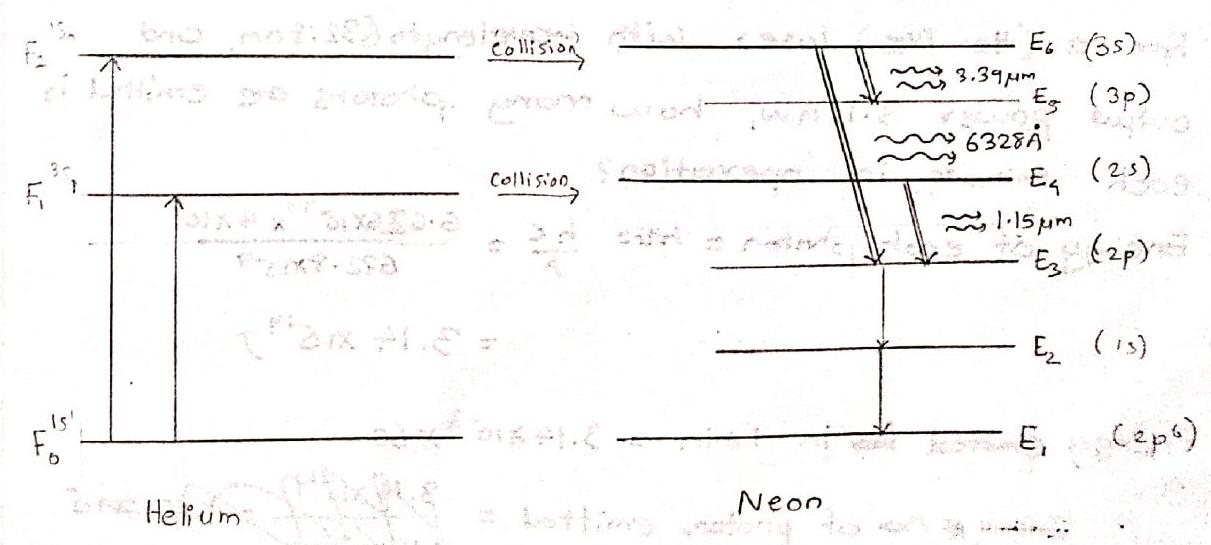
\includegraphics[max width=\textwidth]{2024_06_16_30d750483617f1939202g-04}
\end{center}


\usubsection{Ruby Laser}

\begin{itemize}
	\item first laser fabricated
	\item Created in 1960 by Maiman
	\item It is a 3 level system
	\item Produced light in pulsating maner (continuous mode not possible due to heating of active medium)
	\item Active medium: $\mathrm{Al}_{2} \mathrm{O}_{3} \cdot \mathrm{Cr}^{3+}$ (0.05-0.5 \% of Al atoms are replaced with Cr atoms)
	\item Pumping source: Xenon lamp. (the lamp has a helical structure that wounds the ruby rod).
	\item Eavelength of light emitted: 6943 $\amstr$
\end{itemize}

\begin{center}
	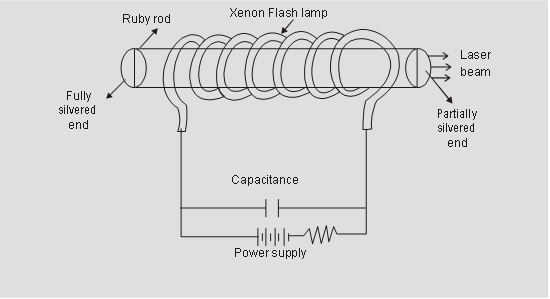
\includegraphics[max width=\textwidth]{ruby-laser}
\end{center}

$\star$ Population inversion is achieved between E$_m$ \& E,
\begin{figure*}
	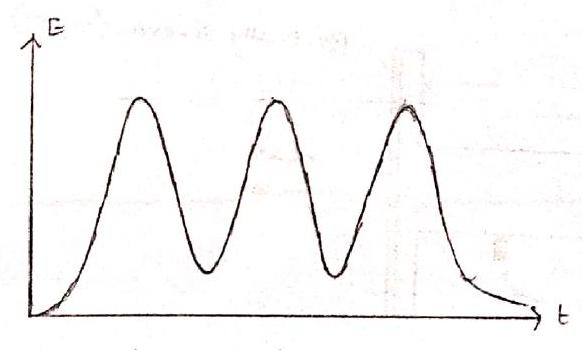
\includegraphics[max width=.5\linewidth]{2024_06_16_30d750483617f1939202g-03}
	\caption*{Intensity us time graph}
\end{figure*}

\ussubsection{Working of Ruby laser}
Cr$^{3+}$ ions absorb pumping light and go to excited states E$_2$ \& E$_3$. From these a rapid non-radiation transition to the metastable level E$_m$ takes place. Decay from E$_m$ is very slow that with sufficient excitation, populations inversion between E$_m$ \& E$_1$ can occur. Those photons are allowed to pass many times in the active medium with the help of mirrors. When threshold conditions are. satisfied, an intense pulse of light of wavelength 6934$\amstr$ is emitted. Continuous operation is not possible due to excessive heating of active medium.

\multiskip{5}

\qa{1}{For semiconductor, band gap is 0.9eV, what is wavelength of light emitted from it?}
{
	\begin{flalign*}
		h\nu               & = 0.9 \unit{eV} = 1.442 \times 10^{-19}\unit{~J}                     &  & \\
		\therefore \nu     & = \frac{1.442 \times 10^{-19}}{h}                                    &  & \\
		                   & = \frac{1.442 \times 10^{-19}}{\h} = 2.176 \times 10^{14} \unit{~Hz} &  & \\
		\therefore \lambda & = c / \nu         = 1.38\unit{~\mu m}                                &  & \\
	\end{flalign*}
}
\qa{2}{For a He-Ne laser with wavelength 632.8 nm and output power 3.14 mW how many photons are emitted in each minute in operation?}
{
	\begin{flalign*}
		\text{Energy of each photon } = h\nu & = \frac{hc}{\lambda}                       &  & \\
		                                     & = \frac{\h \times \lc}{632.8\time 10^{-9}} &  & \\
		                                     & = 3.14 \times 10^{-19} \unit{~J}           &  &
	\end{flalign*}
	\begin{flalign*}
		\therefore \mathrm{ Energy emitted in 1 minute } & = 3.14 \unit{~mW} \times 60 = 0.1884\unit{J}        &  & \\
		\therefore \mathrm{ Number of photons emitted }  & =\frac{0.1884}{3.14 \times 10^{-19}}=6\times10^{17} &  & \\
	\end{flalign*}
}

\qa{3}{Calculate ratio of population of two states of ruby laser in which transition from one state to another is responsible for emission of photon of wavelength 6928 $\amstr$ (Assuming that the transition temperature is 18$^{\circ}$C)}{

	Transition temperature (T) = 18$^{\circ}$C = 291K
	\medskip

	frequency of light emitted $\nu$ = c/$\lambda$ = $\cfrac{\lc}{6928\times 10^{-10}} = 4.3302 \times 10^{14} \unit{Hz}$
	\begin{flalign*}
		\frac{N_2}{N_1} & = e \caret (-h\nu / (kT))                                        &  & \\
		                & = e \caret (-\h \times 4.3302 \times 10^{14} / (\kB \times 291)) &  & \\
		                & = e^{-71.45} = 9.32 \times 10 ^ {-32}                            &  &
	\end{flalign*}
}

\usection{Fibre Optics}
Fibre optics deals with transmission of information using light (which has minimal energy loss). Total internal reflection is the principle behind it.

\usubsection{Total internal reflection}
\textbf{Total internal reflection}: It is a phenomenon which happens when light traveling from denser to lighter medium will reflect back to the same media if the incident angle is greater than a particular angle(known as  critical angle of the media interface).

\begin{minipage}[t][][b]{.57\textwidth}%
	By snell's law:
	$$
		n_{1} \sin \left(\theta_{1}\right)=n_{2} \sin \left(\theta_{2}\right)
	$$

	At critical angle ($\theta_1 = \theta_c$), $\theta_{2}=90$
	\vspace{-.5cm}
	\indentbox{1cm}{
		\begin{flalign*}
			 & \therefore n_{1} \sin \left(\theta_{c}\right)=n_{2}   &  & \\
			 & \theta_{c}=\sin ^{-1}\left(\frac{n_{2}}{n_{1}}\right) &  &
		\end{flalign*}
	}

	\ussubsection{$\theta_c$ for various material interfaces: }
	\begin{itemize}
		\item Water - air =49$^{\circ}$
		\item Diamond - air 24$^{\circ}$
		\item Gluss - air 42$^{\circ}$
	\end{itemize}
\end{minipage}%
\begin{minipage}[t][][b]{.4\textwidth}%
	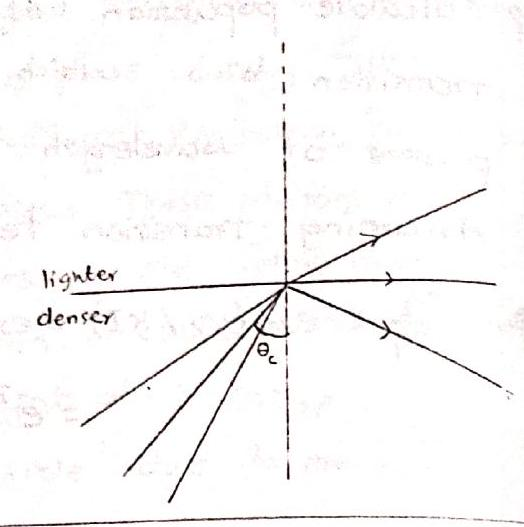
\includegraphics[max width=\textwidth]{2024_06_16_30d750483617f1939202g-05(3)}

	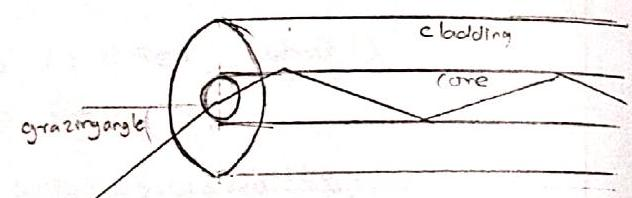
\includegraphics[max width=\textwidth]{2024_06_16_30d750483617f1939202g-05}
\end{minipage}

\usubsection{Structure of Fiber Optic Cable}

\begin{center}
	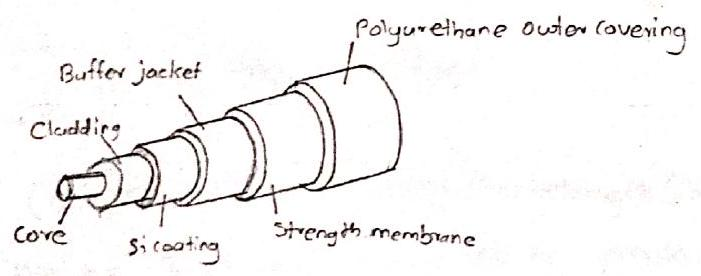
\includegraphics[max width=\textwidth]{2024_06_16_30d750483617f1939202g-05(2)}
\end{center}

\begin{itemize}
	\item Polyurethane: for mecharical crushing
	\item Butfor jacket : to prevent moistume
	\item Si-coarting : protect from dust \& soratches
\end{itemize}


\usubsection{Classification of Fibre Optic Cables}
\begin{itemize}
	\item Based on Index profile: step-index, graded index
	\item Based on made : single mode, multi mode.
\end{itemize}

\ussubsection{Step Index Single Mode}

\begin{center}
	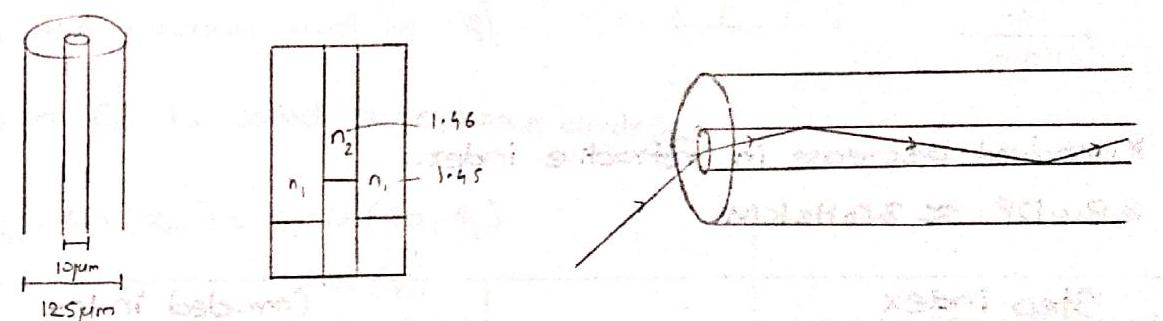
\includegraphics[max width=\textwidth]{2024_06_16_30d750483617f1939202g-05(1)}
\end{center}

\begin{itemize}
	\item Allows only one path for light
	\item Bandwidth distance product: $>3 \unit{GHzkm}$
	\item Splicing is difficut.
\end{itemize}

\ussubsection{Step Index Multi Mode}
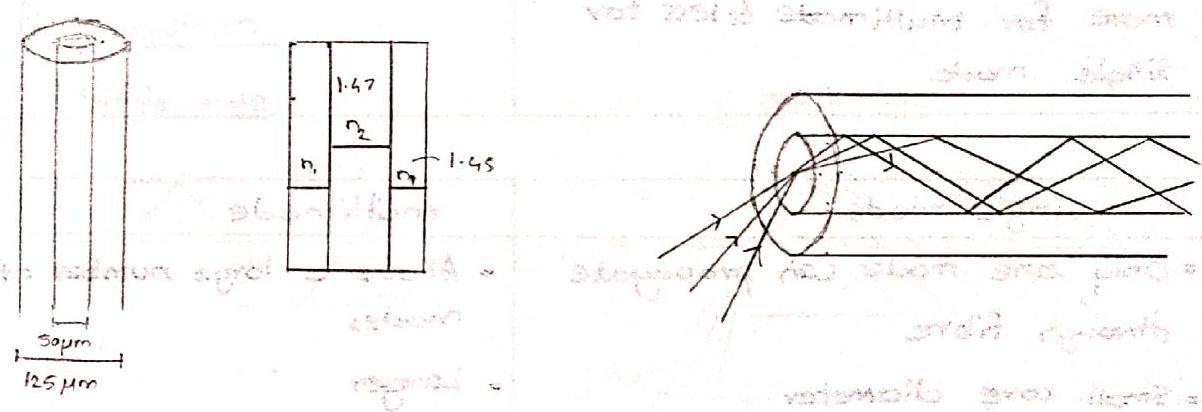
\includegraphics[max width=\textwidth, center]{2024_06_16_30d750483617f1939202g-05(4)}

\begin{itemize}
	\item Allows multiple path for light
	\item easior to splice
	\item Bandwidth distance product (BwDP) $\sim 300 \unit{MHz km}$
\end{itemize}

\ussubsection{Graded Index Multi Mode}

\begin{center}
	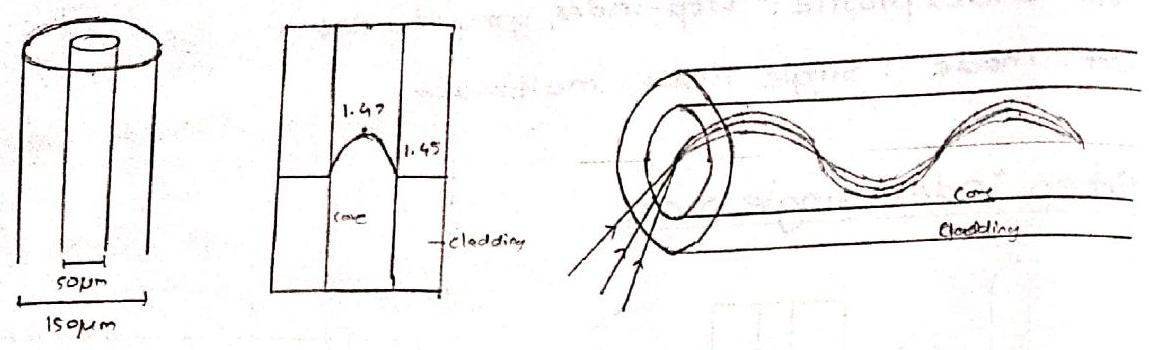
\includegraphics[max width=\textwidth]{2024_06_16_30d750483617f1939202g-06(3)}
\end{center}

\begin{itemize}
	\item Gradual decrease in refractive index.
	\item BWDP $\approx 3 \unit{GHz km}$
\end{itemize}

\ussubsection{Comparison between different Cables}

\begin{longtblr}
	{
		colspec = {XX},
		hlines,
		vlines,
		rowsep=6pt,
		colsep=5pt
	}

	\SetCell{c} \textbf{Step Index}                                   & \SetCell{c} \textbf{Graded Index}                               \\
	Refractive index changes sharply from core-cladding interface     & Refractive index changes gradually from core-cladding interface \\
	Refractive index profile looks like steps                         & Refractive index profile looks like parabola                    \\
	Attenuation is more for multimode and less for single mode        & Attenuation is usually less                                     \\
	Numerical Aperture is more for multimode and less for single mode & Numerical Aperture is usually less                              \\
\end{longtblr}

\begin{longtblr}
	{
		colspec = {XX},
		hlines,
		vlines,
		rowsep=6pt,
		colsep=5pt
	}

	\SetCell{c} \textbf{Single Mode}              & \SetCell{c} \textbf{Multi Mode}                                  \\
	Only one mode can propagate through fibre     & Allows a large number of modes                                   \\
	Smaller core diameter                         & Larger core diameter                                             \\
	Difference in refractive indices is very less & Difference in refractive indices is more compared to single mode \\
	No multimodal dispersion                      & There is multimodal dispersion
\end{longtblr}

\multiskip{2}

\usubsection{Numerical Aperture (NA)}
\begin{minipage}[t][][b]{.67\textwidth}%
	Numerical Aperture is defined as sine of largest angle that a incident ray should have for it to undergo TIR in core
	\bigskip

	By snell's law:
	$n_a\sin (\alpha)=n_1\sin (\alpha)$

	For TIR, angle of incidence	in the medium must be $>\theta_c$.

	$\alpha$ at $\theta_{c}$ is called acceptance angle. $\left(\alpha_{m}\right)$

	\begin{flalign*}
		n_a \sin \left(\alpha_{m}\right) & =n_1 \sin \left(90-\theta_{c}\right)                 &  & \\
		                                 & =n_{1} \cos (\theta)                                 &  & \\
		                                 & \equiv n_{1} \sqrt{1-\sin ^{2}(\theta_c)}            &  & \\
		                                 & =n_{1} \sqrt{1-\left(\frac{n_{2}}{n_{1}}\right)^{2}} &  & \\
		                                 & =\sqrt{n_{1}^{2}-n_{2}^{2}}                          &  &
	\end{flalign*}

	$\boxed{\therefore NA = n_{a} \cdot \sin \left(\alpha_{m}\right) =\sqrt{n_{1}^{2}-n_{2}^{2}}\ }$
\end{minipage}
\begin{minipage}[t][][b]{.3\textwidth}%
	\begin{center}
		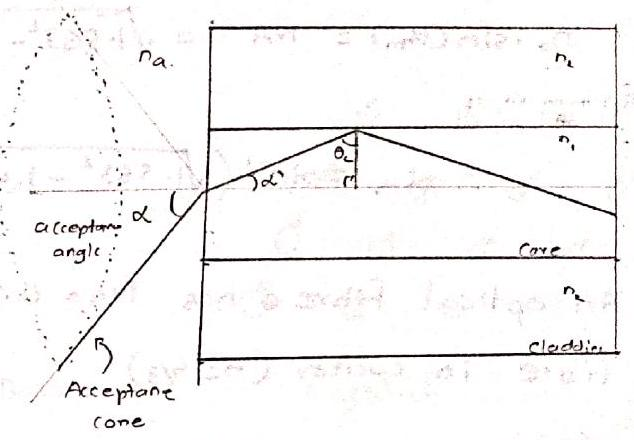
\includegraphics[max width=\textwidth]{2024_06_16_30d750483617f1939202g-06(1)}
	\end{center}

\end{minipage}
\usubsection{Propagation of light ray in Fibre Optic cable}
\begin{minipage}[t][][b]{.67\textwidth}%
	\ussubsection{Single mode \& Multi mode}
	\begin{center}
		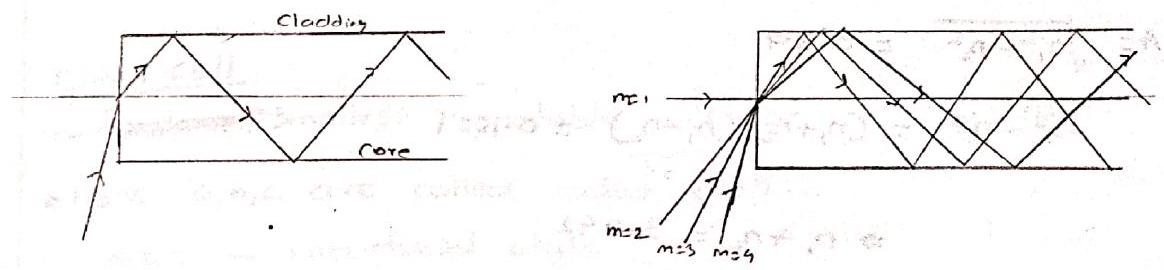
\includegraphics[max width=\textwidth]{2024_06_16_30d750483617f1939202g-06(2)}
	\end{center}
\end{minipage}

\ussubsection{Graded index}

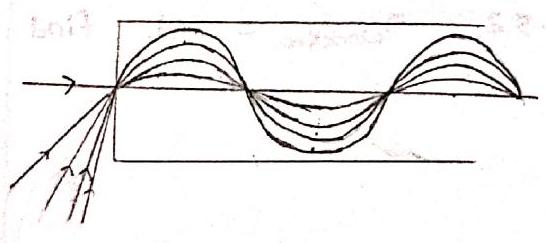
\includegraphics[max width=\floatfigwidth]{2024_06_16_30d750483617f1939202g-06}

$\star$ Eventhough all waves have different velocities, they reach at same time, due to precise differences in distance which they travel.

\qa{1}{An optical fibre has core refractive index of 1.55 \& cladding refractive index of 1.50. Calculate Numerical Aperture}{

	\eqnleft{NA=\sqrt{n_1^2-n_2^2}=\sqrt{1.55^2-1.5^2}=0.391}
}
\qa{2}{Calculate acceptance angle of given fibre, if core refractive index = 1.563 cladding refractive index =1.498}{

	Assuming refractive index of air ($n_a$) = 1.
	\medskip

	\begin{flalign*}
		n_a \cdot \sin \left(\alpha_m\right)           & =\sqrt{1.563^2-1.498^2}                                      &  & \\
		\therefore \text{acceptance angle}\ (\alpha_m) & =\sin ^{-1}\left(\sqrt{1.563^2-1.498^2}\right)=26.49^{\circ} &  & \\
	\end{flalign*}
}

\qa{3}{An optical fibre Numerical Aperture = 0.20, refractive index of cladding = 1.59. Find acceptance angle for fibre in water (n=4/3)}{
	Here $n_a = 4/3$

	\begin{flalign*}
		n_a \sin \left(\alpha_m\right) & =0.20                                                        &  & \\
		\therefore \alpha_m            & =\sin ^{-1}\left(\frac{3}{4} \times 0.20\right)=8.63^{\circ} &  &
	\end{flalign*}
}

\qa{4}{For a cable, Numerical Aperture = 0.39, and difference between refractive indices of core and cladding is 0.05. Find refractive index of core}
{

	\begin{flalign*}
		NA=\sqrt{n_1^2-n_2^2} & =0.39                                                   &  & \\
		n_1^2-n_2^2           & \equiv \left(n_1+n_2\right) \left(n_1-n_2\right)=0.1521 &  &
	\end{flalign*}
	\begin{flalign*}
		\Rightarrow n_1+n_2 & = \frac{0.1521}{n_1-n_2} = 3.042 &  &
	\end{flalign*}
	\begin{flalign*}
		\therefore n_1     =n_{\mathrm{core }} & =\frac{\left(n_1+n_2\right)+\left(n_1-n_2\right)}{2} &  & \\
		                                       & =\frac{3.042+0.05}{2}=1.546                          &  &
	\end{flalign*}
}
\qa{5}{For step index fibre, $n_{\mathrm {core }}=1.52, n_{\mathrm {cladding }}=1.41$. Find $\theta_c$}{
\eqnleft{\theta_c=\sin ^{-1}\left(\frac{1.41}{1.52}\right)=68.1^{\circ}}
}

\end{document}